\chapter{Análisis}

En esta sección, analizamos los datos obtenidos para clasificarlos en Buenos Aires y Córdoba. Tomamos los 260 audios obtenidos a través de la página web y les aplicamos el extractor de atributos descripto en el capítulo 4. El resultado nos dió la descripción de cada grabación a través de los atrbutos que definimos. 

Primero presentamos el baseline que consideramos. El baseline nos sirve para detectar si realizamos una clasificación aceptable. Luego describimos el modelo de testing utilizando los datos recolectados. Explicamos los clasificadores utilizados y en base a test estadísticos notaremos si aportan datos significativos. Por último, analizemos los atributos más descriptivos de cada grupo. Para el análisis de los datos, utilizamos la herramienta Weka\footnote{Página web: http://www.cs.waikato.ac.nz/ml/weka/}. Esta nos provee varios algoritmos de Machine Learning. 

\section{Baseline}

No hay ningún trabajo que trate de distinguir entre porteños y cordobéces a partir de su habla. Es por eso que definimos el baseline utilizando el algoritmo \textbf{majority class}. Este algoritmo, utilizando nuestros datos, tendría una performance buena. En nuestro caso estará llegando al 45\% de efectividad aproximadamente. Este es el porcentaje a superar. 

%Pensemos que para determinar si una persona corresponde a alguno de los grupos vamos a tirar una moneda. Empíricamente podemos afirmar que en promedio la probabilidad de que salga algún grupo es 1/2. Gracias a la Ley de los Grandes Números podemos afirmar que, para valores grandes, esto va a tender a la Esperanza. Entonces, si nosotros queremos identificar un hablante utilizando el azar nos dará el 50\% de efetividad.

%Cabe aclarar que nuestro set de datos no esta debidamente balanceado. Tuvimos más grabaciones de Buenos Aires que de Córdoba. Es por eso que el entrenamiento también va a ser desbalanceado. Por este motivo puede suceder que al clasificar a un hablante en un test se obtenga mejores resultados para características de Buenos Aires que de Córdoba. Lamentablemente eso es una problemática de los datos obtenidos.

Cabe aclarar que, si nuestro set de datos estuviera debidamente balanceado este porcentaje no sería tan alto. Lo ideal sería poder tener muestras balanceadas. Al tener este desbalance, puede suceder que al clasificar a un hablante en un test se obtenga mejores resultados para características de Buenos Aires que de Córdoba. Lamentablemente esto es una problemática de los datos obtenidos.

La herramienta Weka provee un clasificador basado en mayority class llamado \textbf{ZeroR}. Utilizaremos este para el cálculo del baseline. 

\section{Modelo de testing}

La complejidad del problema y la forma en que fue realizado el experimento nos llevó a tener que descartar un modelo de testing común. Si utilizamos un modelo estándar deberíamos dividir los audios en dos grupos, uno lo usaríamos para entrenar y otro para testear. En este contexto, podría surgir el problema de que un hablante tenga audios en el conjunto de train y también en el de test. En ese caso el test sería erróneo ya que estaríamos entrenando con datos que luego serían testeados.

Para evitar este inconveniente debimos tomar en cuenta los hablantes a la hora de dividir los grupos. Dividimos \textbf{a los hablantes} en dos conjuntos: uno llamado train que se utiliza para entrenar, y otro test que testea el clasificador entrenado. Si bien esto evita el problema anterior, la cantidad de audios aportados por cada hablante es muy variable. Un hablante pudo haber aportado 30 grabaciones mientras que otro sólo pudo haber realizado 5. Tomando en cuenta esto, la cantidad de audios de un grupo con respecto a otro puede quedar muy desbalanceada. Para mitigar este problema, tomamos que el conjunto de train tenga el 70\% de las instancias mientras que el restante 30\% sea destinado para test. Estos dos grupos conformaron un conjunto de test. 

No podemos quedarnos con uno sólo conjunto de test, ya que haría encasillar a cada hablante en el conjunto de train o de test. Es por esto que creamos 5 conjuntos de test. En definitiva, creamos 5 conjuntos de test de la forma $<$train, test$>$ con las características antes descriptas. A esto lo llamamos \textbf{cross-validation test}. 

Otro problema a tener en cuenta es que los grupos de test generados sean lo más distintos posibles. Para solucionar esto, el test de cross-validation fue de la siguiente forma: armamos conjuntos a partir de las instancias para train y test, pero con una salvedad. Para armar el conjunto de test utilizarmos el 20\% de los elementos de las instancias ya utilizadas en los tests anteriores y el resto de instancias nuevas. De esta forma, regulamos la cantidad de instancias repetidas en los tests y nos aseguramos que sean todos distintos. Esto nos permitió utilizar instancias nuevas en los 5 conjuntos. 

A continuación el código generador del test cross-validation:
\lstset{ %
language=C++,                % choose the language of the code
basicstyle=\footnotesize,       % the size of the fonts that are used for the code
numbers=left,                   % where to put the line-numbers
numberstyle=\small,      % the size of the fonts that are used for the line-numbers
stepnumber=1,                   % the step between two line-numbers. If it is 1 each line will be numbered
numbersep=5pt,                  % how far the line-numbers are from the code
backgroundcolor=\color{white},  % choose the background color. You must add \usepackage{color}
showspaces=false,               % show spaces adding particular underscores
showstringspaces=false,         % underline spaces within strings
showtabs=false,                 % show tabs within strings adding particular underscores
frame=lines,           % adds a frame around the code
tabsize=1,          % sets default tabsize to 2 spaces
captionpos=b,           % sets the caption-position to bottom
breaklines=true,        % sets automatic line breaking
postbreak=\raisebox{0ex}[0ex][0ex]{\ensuremath{\hookrightarrow\space}},
breakatwhitespace=false,    % sets if automatic breaks should only happen at whitespace
escapeinside={\%*}{*)},          % if you want to add a comment within your code
morekeywords={GeneradorDeTest, porcentajeMaximoDeSimilitud, checkBalance, Input, Output, Repetir, veces, Si, Agregar, Recorrer, Devolver, y, no, esta, en},
literate= {<-} {$\le$}{2} {!=} {$\neq$}{2} {<-} {$\leftarrow$}{2} {==} {=}{2} {&&} {$\cap$}{2} {||} {$\cup$}{2} }
\begin{lstlisting}
    GeneradorDeTest:
    Input: conjunto audios
    Output: conjunto de <train, test>
    resultado <- {} 
    train <- {}
    test <- {}
    hablantesEnTests <- {}
    hablantes <- ObtenerHablantes(audios)
    tamTest <- tam(hablantes) * 0.3
    Repetir 5 veces:
        hablantesUsadosEnTest <- ElegirRandom(hablantesEnTest, tamTest * 0.2)
        hablantesNoUsadosEnTest <- ElergirRandom(hablantes - hablantesEnTest, tamTest * 0.8)
        hablantesTest <- hablantesEnTest + hablantesNoUsadosEnTest

        test <- ObtenerAudios(hablantesTest, audios)

        train <- ObtenerAudios(hablantes - hablantesTest, audios)

        Si <train, test> no esta en resultado y 
           porcentajeMaximoDeSimilitud(test, resultado, 0.2) y
           checkBalance(train) y checkBalance(test):
              Agregar <train, test> a resultado
              Agregar hablantesTest a hablantesEnTests
    Devolver resultado
    
    porcentajeMaximoDeSimilitud(conj, resultado, 0.2):
    Input: conj, conjunto de <train, test>, pct
    Output: booleano
    Recorrer test de conjunto de <train, test>:
    	pct <- Maximo(pct, porcentajeSimilitud(conj, test))
    Devolver pct < 0.2	

    checkBalance:
    Input: conj, pct
    Output: booleano
    bool_bsas <- #(conj) * 0.55 < #bsas(conj) < #(conj) * 0.65
    bool_cba <- #(conj) * 0.45 < #cba(conj) < #(conj) * 0.45
    Devolver bool_bsas y bool_cba
\end{lstlisting}

En las lineas 11 y 12, agregamos los hablantes usados en los test anteriores y luego los nuevos hablantes todavía no utilizados. Luego  en las lineas 15 y 17, de esos hablantes obtenemos los datos extraídos de sus audios. Finalmente chequeamos las últimas características: que el par generado no sea uno ya previamente generado, que el conjunto test sólo tenga como máximo 20\% de elementos repetidos de los demás tests (lineas 20 y 26) y que el balance de Córdoba y de Buenos Aires sea aproximadamente de un 40\% y 60\% respectivamente.

A continuación veremos los clasificadores que utilizaremos para predecir qué lugar pertenece cada hablante.

\section{Clasificadores}

Entrenamos varios clasificadores para poder determinar la procedencia de un hablante y mejorar la performance del baseline. Los clasificadores propuestos son: 

\paragraph{Repeated Incremental Pruning to Produce Error Reduction (RIPPER) \cite{Cohen1995} - Implementación JRip:}

%http://weka.sourceforge.net/doc.dev/weka/classifiers/rules/JRip.html
%http://www.cs.utsa.edu/~bylander/cs6243/cohen95ripper.pdf
%https://indico.cern.ch/event/34666/session/13/material/slides/0?contribId=16 pag 21

Este algoritmo intenta describir el conjunto de entrada definiendo pequeños grupos. Primero localiza un grupo que posee la característica a clasificar, y genera reglas que lo describan. Va agregando reglas de forma golosa. Luego cuando se supera una cierta condición (por ejemplo: cantidad de reglas), lo extrae y sigue con otro grupo. Finaliza cuando describe todos los grupos del conjunto de entrada. Este algoritmo sirve mucho para datos no balanceados.

\paragraph{C4.5 \cite{Quinlan1993} - Implementación J48:}

%http://en.wikipedia.org/wiki/C4.5_algorithm
%http://weka.sourceforge.net/doc.dev/weka/classifiers/trees/J48.html

Este algoritmo se basa en un árbol de decisión. Dada una serie de muestras con varios atributos se realiza lo siguiente: para cada atributo calcula su ganancia de información. Elige el que tenga mejor ganancia entre todos los atributos y con él crea un nodo en el árbol. Aplica recursivamente por cada rama. Si las muestras pertenecen a la misma clase o los atributos no proveen información se crea solo una hoja.

\paragraph{Support Vector Machines \cite{Platt98sequentialminimal} - Implementación Function SMO:}

%http://en.wikipedia.org/wiki/Support_vector_machine
%http://machinelearning.wustl.edu/mlpapers/paper_files/BordesEWB05.pdf
%http://en.wikipedia.org/wiki/Sequential_minimal_optimization
%http://research.microsoft.com/pubs/69644/tr-98-14.pdf

Support vector machines define uno o varios hiperplanos para intentar clasificar muestras. Este hiperplano se construye utilizando combinaciones lineales de los datos de entrada y sirve para clasificar las muestras en los dos grupos de la mejor forma posible. Utilizando este hiperplano, se puede etiquetar cada dato de entrada con su clasificación observando de qué lado del hiperplano se encuentra.

\paragraph{Naive Bayes \cite{DBLP:conf/flairs/Zhang04} - Implementación homónima:}

%http://www.cs.unb.ca/profs/hzhang/publications/FLAIRS04ZhangH.pdf
%http://en.wikipedia.org/wiki/Naive_Bayes_classifier

Un clasificador de tipo Naive Bayes asume que cada atributo describe una característica de su clase y no esta relacionado con otro atributo. Cada uno de estos atributos contribuye de manera independiente a la clasificación de su clase. Se define una regla de decisión utilizando un modelo probabilístico basado en el teorema de Bayes para la clasificación de cada grupo.

\section{Tests estadísticos}

Utilizamos los resultados de cada clasificador para ver si son significativamente relevantes en la predicción de cada hablante en comparación con el baseline. Los resultados que utilizamos son el vector resultante de entrenar con train y clasificar con test para los 5 grupos de test generados. Los clasificadores utilizados son ZeroR, o sea el baseline, comparado con algún clasificador más sofisticado, por ejemplo: JRip, J48, Function SMO y NaiveBayes. Para estos resultados realizarmos dos principales tests: Wilcoxon signed-rank y Test de Student. 

\subsection{Wilcox Test}

Primero realizamos Wilcox Test ya que no estamos seguro que nuestros datos provengan de una distribucón Normal. Para realizar este test debemos cumplir que:

\begin{itemize}
    %Data are paired and come from the same population.
    \item Los datos son presentados de a pares y vienen de la misma población: esto sucede gracias a como generamos los tests. La población también siempre es la misma.
    %Each pair is chosen randomly and independently.
    \item Cada par es elegido al azar y independiente del resto: cada grupo generado para testing esta armado de forma azarosa ya que la elección de cada hablante se realiza de esta forma.
    %The data are measured at least on an ordinal scale, but need not be normal.
    \item Los datos están medidos sobre una escala ordinal y no necesariamente debe provenir de una distribución Normal: esta característica es fundamental ya que, como dijimos, no estamos seguros que nuestros datos provengan de una distribución Normal.
\end{itemize}

El input del mismo fue el vector resultante del test baseline ZeroR con el vector de los demás clasificadores. Las hipótesis fueron:

\vspace{0.5cm}
\hspace{2cm}Ho: Clasificador alternativo no es mejor que ZeroR
\vspace{0.25cm}

\hspace{2cm}H1: Clasificador alternativo es mejor que ZeroR
\vspace{0.5cm}

Clasificador alternativo se refiere a los demás clasificadores descriptos. Cada uno de los tests nos va a dar un p-valor. Si este es mayor 0,05, no hay evidencia suficiente para determinar que el clasificador alternativo es mejor. Si de lo contrario es menor, sí podemos rechazar Ho y asegurar que el alternativo es mejor. 

Luego chequeamos si nuestra muestra corresponde a una distribución Normal. Para chequear Normalidad utilizamos el test de Shapiro-Wilk.

\subsection{Análisis Shapiro-Wilk Test}

%todo: pensar si debo explicar todo el metodo o no hace falta
%http://es.wikipedia.org/wiki/Test_de_Shapiro%E2%80%93Wilk

%En estadística, el Test de Shapiro–Wilk se usa para contrastar la normalidad de un conjunto de datos. Se plantea como hipótesis nula que una muestra x1, ..., xn proviene de una población normalmente distribuida. Fue publicado en 1965 por Samuel Shapiro y Martin Wilk.1 Se considera uno de los test más potentes para el contraste de normalidad, sobre todo para muestras pequeñas (n<30).

El Test de Shapiro-Wilk lo utilizamos para poder afirmar si conjunto de datos proviene de una distribución Normal. Una característica importante es que posee un buen desempeño en pequeñas muestras.

%Interpretación: Siendo la hipótesis nula que la población está distribuida normalmente, si el p-valor es menor a alfa (nivel de confianza) entonces la hipótesis nula es rechazada (se concluye que los datos no vienen de una distribución normal). Si el p-valor es mayor a alfa, no se rechaza la hipótesis y se concluye que los datos siguen una distribución normal.

El test de Shapiro-Wilk se basa en plantear como hipótesis nula que la población esta distribuida de forma Normal. Aplicamos el estadístico de este test: si el p-valor nos da menor a 0,05 entonces la hipótesis nula es rechazada y se afirma que los datos no provienen de una distribución Normal. Si, en cambio, es mayor a 0,05 no se puede rechazar Ho y por ende se afirma que los datos siguen una distribución Normal.

Este test se realiza individualmente para cada vector resultado. O sea, chequeamos que los resultados de cada clasificador se asemejen a la distribución Normal. Por ejemplo si los resultados de ambos clasificadores ZeroR y J48 tuvieron en el test Shapiro-Wilk un p-valor mayor a 0,05, se puede realizar el Student Test para ellos dos. 

\subsection{Student Test}

%En estadística, una prueba t de Student, prueba t-Student, o Test-T es cualquier prueba en la que el estadístico utilizado tiene una distribución t de Student si la hipótesis nula es cierta. Se aplica cuando la población estudiada sigue una distribución normal pero el tamaño muestral es demasiado pequeño como para que el estadístico en el que está basada la inferencia esté normalmente distribuido, utilizándose una estimación de la desviación típica en lugar del valor real. Es utilizado en análisis discriminante.

%A t-test is any statistical hypothesis test in which the test statistic follows a Student's t distribution if the null hypothesis is supported. It can be used to determine if two sets of data are significantly different from each other, and is most commonly applied when the test statistic would follow a normal distribution if the value of a scaling term in the test statistic were known. When the scaling term is unknown and is replaced by an estimate based on the data, the test statistic (under certain conditions) follows a Student's t distribution.

Para los vectores que poseen una distribución Normal aplicamos este test. Este nos provee una forma de determinar si dos conjuntos de test son significativamente distintos. De la misma forma que planteamos la hipótesis de Wilcox test, este va a tener las mismas hipótesis. O sea: 

\vspace{0.5cm}
\hspace{2cm}Ho: Clasificador alternativo no es mejor que ZeroR
\vspace{0.25cm}

\hspace{2cm}H1: Clasificador alternativo es mejor que ZeroR
\vspace{0.5cm}

La ventaja de usarlo es que, al saber que distribución representa, vamos a tener resultados mas precisos. Aplicando el estadístico obtuvimos un p-valor. De la misma forma, si este es mayor a 0,05 no hay evidencia suficiente para rechazar Ho. De lo contrario, si hay evidencia y rechazamos Ho.

\section{Resultados}

Recordemos que al tener pocos datos debimos repetir instancias en los grupos de tests. El porcentaje de instancias repetidas es menor al 20\%. Vamos a mostrar como son estos conjuntos:

\begin{figure}[H]
\centering
\pgfplotsset{width=10cm, height=6cm}
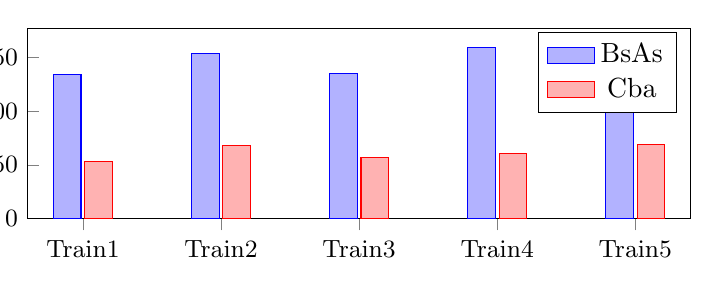
\begin{tikzpicture}[trim axis left, trim axis right]
\begin{axis}[
    ybar,
    tick label style={font=\small},
    tickpos=left,
    xticklabels={Train1, Train2, Train3, Train4, Train5}, 
    xtick={1,2,3,4,5},
    ymin=0,
    legend entries={BsAs,Cba},
    ]
    \addplot +[bar shift=-.2cm, area legend] coordinates {(1,134) (2,154) (3,135) (4,159) (5,161)};

    \addplot  +[bar shift=.2cm, area legend]coordinates {(1,53) (2,68) (3,57) (4,61) (5,69)};
\end{axis}
\end{tikzpicture}
\end{figure}

\begin{figure}[H]
\centering
\pgfplotsset{width=10cm, height=4cm}
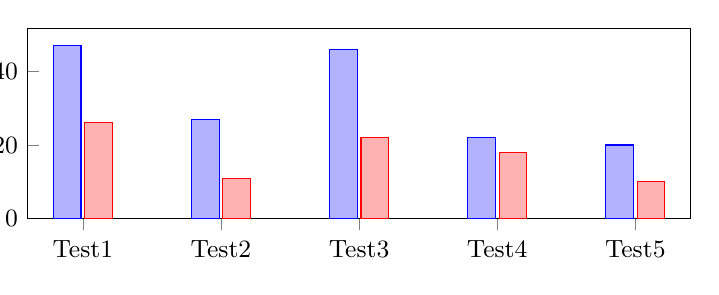
\begin{tikzpicture}[trim axis left, trim axis right]
\begin{axis}[
    ybar,
    tick label style={font=\small},
    tickpos=left,
    xticklabels={Test1, Test2, Test3, Test4, Test5}, 
    xtick={1,2,3,4,5},
    ymin=0,
    ]
    \addplot +[bar shift=-.2cm, area legend] coordinates {(1,47) (2,27) (3,46) (4,22) (5,20)};

    \addplot  +[bar shift=.2cm, area legend]coordinates {(1,26) (2,11) (3,22) (4,18) (5,10)};
\end{axis}
\end{tikzpicture}
\caption{Cantidad de instancias de Buenos Aires y Córdoba según cada grupo de Train y Tests}
\label{TestsInstances}
\end{figure}

Los resultados en porcentaje para los distintos clasificadores fueron:

\begin{table}[H]
\centering
\begin{tabular}{|l|c|c|c|c|c|c|}
\hline
\textbf{}  & \textbf{ZeroR} & \textbf{JRip} & \textbf{J48} & \textbf{Function SMO} & \textbf{NaiveBayes} \\ \hline
\textbf{Test 1}  & 64 & 61 & 64 & 73 & 63 \\ \hline
\textbf{Test 2}  & 71 & 68 & 71 & 76 & 71 \\ \hline
\textbf{Test 3}  & 67 & 54 & 45 & 75 & 67 \\ \hline
\textbf{Test 4}  & 55 & 52 & 55 & 67 & 80 \\ \hline
\textbf{Test 5}  & 66 & 70 & 66 & 70 & 70 \\ \hline
\hline \hline
\textbf{Promedio} & 64 & 61 & 60 & 72 & 70 \\ \hline
\end{tabular}
\end{table}

Donde Test 1 corresponde al primer par $<$train, test$>$ y así sucesivamente. En la figura \ref{porcentajexClasificador} se puede ver el porcentaje de cada tests en comparación. Excluimos a JRip y J48 por dar muy parecido a ZeroR.

\begin{figure}[H]
\centering
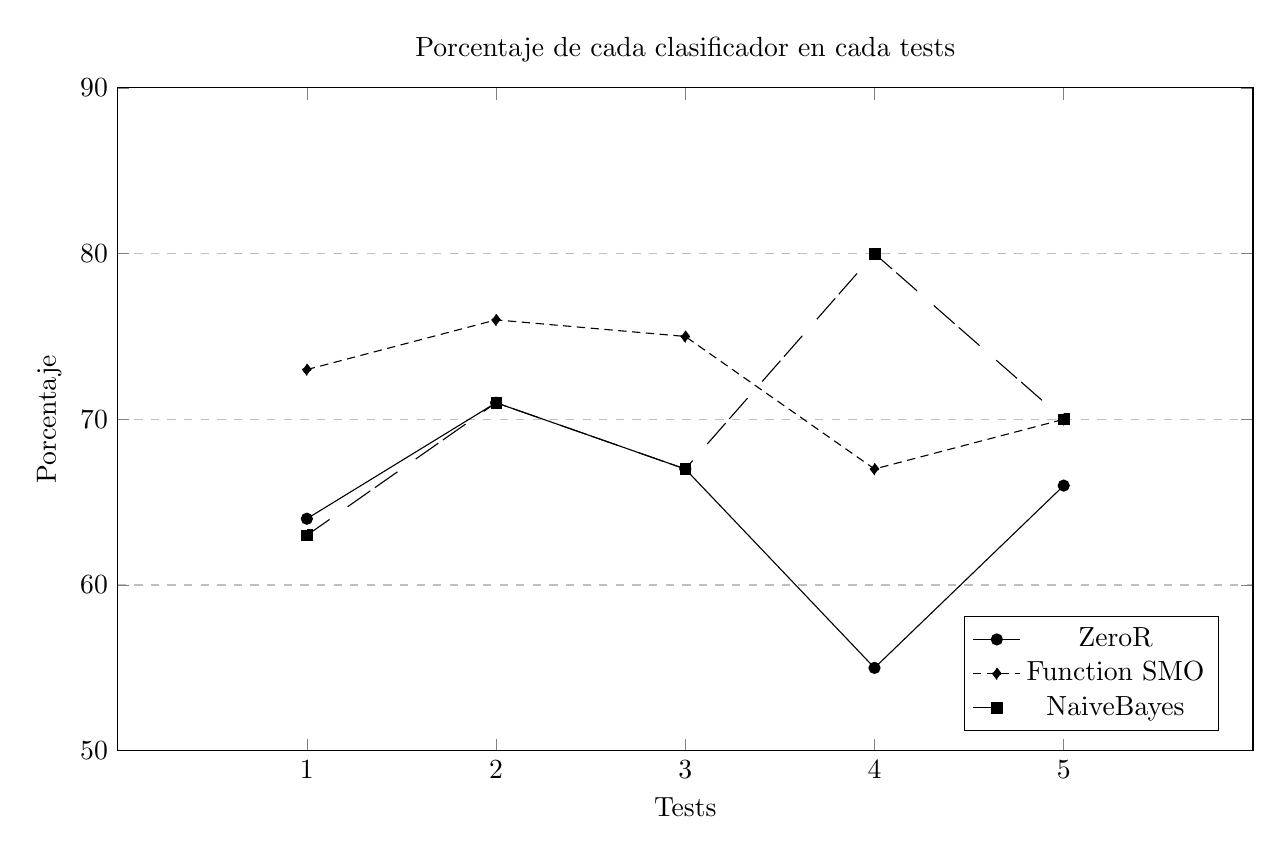
\begin{tikzpicture}
\begin{axis}[
	width=16cm,
	height=10cm,
    title={Porcentaje de cada clasificador en cada tests},
    xlabel={Tests},
    ylabel={Porcentaje},
    xmin=0, xmax=6,
    ymin=50, ymax=90,
    xtick={1,2,3,4,5},
    ytick={20,30,40,50,60,70,80,90,100},
    legend pos=south east,
    ymajorgrids=true,
    grid style=dashed
] 
\addplot [mark=otimes*, width=1pt] coordinates {
    (1,64)(2,71)(3,67)(4,55)(5,66) };\addlegendentry{ZeroR};
%\addplot[mark=diamond*,dash pattern=on 10pt off 2pt on 3pt off 2pt]coordinates {
%    (1,61)(2,68)(3,54)(4,52)(5,70) };\addlegendentry{JRip};
\addplot [mark=diamond*,dash pattern=on 3pt off 2pt on 3pt off 2pt]coordinates {
    (1,73)(2,76)(3,75)(4,67)(5,70) };\addlegendentry{Function SMO};
\addplot [mark=square*,dash pattern=on 10pt off 8pt on 10pt off 2pt]coordinates {
    (1,63)(2,71)(3,67)(4,80)(5,70) };\addlegendentry{NaiveBayes};
\end{axis}
\end{tikzpicture}
\caption{Porcentaje de ZeroR, Function SMO y NaiveBayes}
\label{porcentajexClasificador}
\end{figure}

Recordemos que el clasificador ZeroR elige siempre la clase mayoritaria en su grupo de test. Viendo la figura \ref{porcentajexClasificador} podemos notar que ZeroR mantiene un porcentaje en los diferentes tests entre un 55\% y casi 70\%. El clasificador Function SMO siempre se mantiene por arriba de este baseline. 

Algo interesante sucede con el clasificador Function SMO: posee métricas muy similares a ZeroR pero en el test 4 posee mucha mejor performance. Viendo los grupos generados en la figura \ref{TestsInstances}, el test 4 es el que tiene menos diferencia entre cantidad de hablantes de Buenos Aires y Córdoba. Al tener mitad instancias de cada grupo y como ZeroR elige entre uno de esos dos, va a poseer un porcentaje de acierto cercano al 50\%, como sucede.  

El porcentaje de exactitud en la clasificación se puede apreciar con la métrica \textit{Precision} y \textit{Recall}. \textit{Precision} se define como la cantidad de verdaderos positivos sobre la cantidad de verdaderos y falsos positivos. \textit{Recall} se define como la cantidad de verdaderos positivos sobre la cantidad de verdaderos positivos y falsos negativos. Tomamos como verdaderos positivos a la condición de que fue clasificado como Buenos Aires y efectivamente es de ahí. Falsos negativos si el hablante es de Buenos Aires pero es clasificado como Córdoba. Y falso positivo si el hablante es de Córdoba pero es clasificado como Buenos Aires. 

%http://en.wikipedia.org/wiki/Precision_and_recall

Estos valores surgen de la matriz de confusión. Vamos a analizar como son estas métricas para el caso del test 4, que es el más interesante.

% Precision = VP / VP + FP
% Recall = VP / VP + FN
% VP = "BsAs classif. como BsAs"
% FN = "BsAs classif. como Cba"
% FP = "Cba classif. como BsAs" 

\paragraph*{ZeroR:}\mbox{}\\
\begin{table}[H]
\centering
\begin{tabular}{|c|c|l|c|c|c|c|}
\hline
 BsAs & Cba &  \\ \hline
 22 &  18 &  Clasificado como BsAs \\ \hline
 0  &   0 &  Clasificado como Cba \\ \hline
\end{tabular}
\end{table}
\begin{center}
\textbf{Precision = 22/40 = 0.55;} \textbf{Recall = 1}\\
\textbf{Instancias correctas = 55\%}
\end{center}

\paragraph*{Function SMO:}\mbox{}\\
\begin{table}[H]
\centering
\begin{tabular}{|c|c|l|c|c|c|c|}
\hline
 BsAs & Cba &  \\ \hline
 22 &  13 &  Clasificado como BsAs \\ \hline
 0  &   5 &  Clasificado como Cba \\ \hline
\end{tabular}
\end{table}
\begin{center}
\textbf{Precision = 22/35 = 0.63;} \textbf{Recall = 1}\\
\textbf{Instancias correctas = 67\%}
\end{center}

\paragraph*{NaiveBayes:}\mbox{}\\
\begin{table}[H]
\centering
\begin{tabular}{|c|c|l|c|c|c|c|}
\hline
 BsAs & Cba &  \\ \hline
 20 &  6 &  Clasificado como BsAs \\ \hline
 2  &  12 &  Clasificado como Cba \\ \hline
\end{tabular}
\end{table}
\begin{center}
\textbf{Precision = 20/26 = 0.77;} \textbf{Recall = 20/22 = 0.9}\\
\textbf{Instancias correctas = 80\%}
\end{center}

Viendo estas matrices de confusión y sus métricas podemos observar cuál es el error que se produce en cada uno de los clasificadores. Notamos que ZeroR produce mucho \textit{Error de tipo I} ( clasificador afirma que es de Buenos Aires y en realidad es de Córdoba). Esto sucede ya que elige solo una categoría siempre. En los demás clasificadores se intenta realmente predecir y por eso los Errores de tipo I y II están mas distribuidos.

Otro dato a tener en cuenta es que si bien, el clasificador ZeroR tuvo un valor alto en la métrica \textit{Recall}, no fue lo mismo para \textit{Precision} y por eso el valor de instancias correctas dio bastante malo. Ambos valores deben estar cercanos al 1 para tener una buena performance. Por eso en el caso de NaiveBayes; si bien ningún valor dio 1, ambos están cerca y posee en mayor porcentaje de instancias correctas.

Puede suceder que el porcentaje de instancias correctas sea el mismo pero los Errores de tipo I y II sean más balanceados. Esto es el caso del conjunto de test 1. Este caso para los clasificadores ZeroR y NaiveBayes es:

\paragraph*{ZeroR:}\mbox{}\\
\begin{table}[H]
\centering
\begin{tabular}{|c|c|l|c|c|c|c|}
\hline
 BsAs & Cba &  \\ \hline
 47 &  26 &  Clasificado como BsAs \\ \hline
 0 &  0 &  Clasificado como Cba \\ \hline
\end{tabular}
\end{table}
\begin{center}
\textbf{Precision = 47/73 = 0.64;} \textbf{Recall = 47/47 = 1}\\
\textbf{Instancias correctas = 64\%}
\end{center}

\paragraph*{NaiveBayes:}\mbox{}\\
\begin{table}[H]
\centering
\begin{tabular}{|c|c|l|c|c|c|c|}
\hline
 BsAs & Cba &  \\ \hline
 33 &  13 &  Clasificado como BsAs \\ \hline
 14 &  13 &  Clasificado como Cba \\ \hline
\end{tabular}
\end{table}
\begin{center}
\textbf{Precision = 33/46 = 0.7;} \textbf{Recall = 33/47 = 0.7}\\
\textbf{Instancias correctas = 63\%}
\end{center}

En este caso notamos que, a pesar de que el porcentaje de instancias correctas den valores cercanos, ZeroR concentra grán parte del error en un tipo sólo, mientras que NaiveBayes lo distribuye entre los dos tipos.

\subsection{Wilcox y Student Test}

En esta sección mostramos los resultados de estos tests estadísticos. Todos los tests estadísticos realizados fueron realizados utilizando R versión 3.0.1. Recordemos que los resultados surgieron de realizar los test de Wilcox y Student para el vector resultado de cada clasificador con respecto a ZeroR.

\begin{table}[H]
\centering
\begin{tabular}{|l|c|c|c|c|c|c|}
\hline
\textbf{}  & \textbf{Student Test} & \textbf{Wilcox Test} \\ \hline
\textbf{ZeroR y JRip}  & 0.8438 & 0.87 \\ \hline
\textbf{ZeroR y J48}  & 0.9772 & 0.813 \\ \hline
\textbf{ZeroR y NaiveBayes}  & 0.2113 & 0.1692 \\ \hline
\textbf{ZeroR y Function SMO}  & 0.03125 & 0.004545 \\ \hline
\end{tabular}
\end{table}

Todos los clasificadores pasaron el test Shapiro-Wilk, entonces podemos afirmar que los resultados de cada clasificador corresponden a una distribución Normal. Analizando estos resultados notamos que para el clasificador Function SMO posee p-valor menor a 0,05 en ambas columnas. Esto quiere decir que \textbf{Function SMO tiene evidencia suficiente para ser mejor que ZeroR}. Por otro lado, los demás no pudieron lograr este cometido. 

\subsection{Clasificadores encontrados}

Analizamos la salida del clasificador JRip ya que, de los clasificadores elegidos, es el que utiliza una cantidad manejable de atributos. Los demás clasificadores utilizaron muchos más atributos y por ende debimos descartarlos ya que el análisis se tornaba engorroso. 

Cada conjunto de test devolvió un conjunto de reglas y no fueron necesariamente iguales entre sí. Estos datos corresponden a la clasificación $train 0$ y $test 0$.

\paragraph*{Clasificador JRip:}

\begin{flushleft}
\begin{itemize}

\item $(FON\_ll\_norm <= -11.08) and (ACU\_AverageLL\_6 <= 4.308) => place=cba (12.0/0.0)$ \\
\item $(FON\_Sfinal\_normhd <= 27.874) and (SIL\_prevSyllableAccent\_norm >= -4.265) => place=cba (11.0/1.0)$ \\
\item $(FON\_rr\_normhd <= 31.355) => place=cba (10.0/2.0)$ \\
\item $ else  => place=bsas (154.0/23.0)$
\end{itemize}
\end{flushleft}

Podemos notar en el anterior árbol de decisión que la duración sobre /ll/, el estiramiento de la /s/ al final de la palabra, la duración sobre /r/ y la duración de la sílaba anterior a la acentuada fueron los elegidos para clasificar los dos grupos. Si bien este clasificador no obtuvo buena performance, analizar su árbol de decisión nos permite pensar cuales atributos tienen mayor importancia a la hora de la clasificación.

Analizamos a continuación cuales atributos aportan mayor información.

\section{Selección de atributos de forma automática}

En esta sección aplicaremos a los distintos atributos evaluadores para analizar cual posee mayor importancia. 

\subsection*{Attribute Evaluator: InfoGain}
%http://weka.sourceforge.net/doc.dev/weka/attributeSelection/InfoGainAttributeEval.html

El evaluador utilizado fue InfoGain para analizar la importancia de cada atributo y utilizamos Ranker para el puntaje de los atributos. Estos algoritmos trabajan de la siguiente forma: para cada atributo calcula la entropía de la clase y luego se calcula la entropía de la misma sabiendo que ese atributo se cumple. La ganancia de información de ese atributo es la resta de esos dos resultados. Esto se puede expresar como: $InfoGain(Class,Attribute) = H(Class) - H(Class | Attribute)$. De esta forma, cuanto menor sea la entropía sabiendo ese atributo mayor será la ganancia de información para ese atributo.

\begin{table}[H]
\centering
\begin{tabular}{|c|l|c|c|c|c|c|}
\hline
 0.07231     & FON\_consonant\_norm \\ \hline
 0.07217     & FON\_vowel\_norm \\ \hline
 0.03963     & SIL\_syllableAccent\_normhd \\ \hline
 0.03963     & SIL\_prevSyllableAccent\_normhd \\ \hline
 0.02332     & FON\_ll\_norm \\ \hline
 0.02285     & FON\_Sfinal\_norm \\ \hline
 0.02226     & ACU\_MinLL\_1 \\ \hline
 0.02144     & ACU\_AverageLL\_1 \\ \hline
 
\end{tabular}
\end{table}

Analizando los resultados vemos que los más preponderantes se refieren a la duración de consonantes, vocales, duración de la sílaba acentuada y su sílaba anterior. El atributo sobre la duración de la sílaba y su anterior es entendible que aporte la mayor ganancia de información ya que es la característica conocida para distinguir los dos grupos. No es extraño encontrarlos entre los primeros lugares. 

Los atributos sobre duración de consonantes y vocales sorprenden con sus valores pero luego de analizarlos son entendibles. Todas las reglas definidas, salvo la regla 1 sobre estirar la sílaba anterior a la acentuada, están definidas utilizando consonantes. Vocales también pero en menor medida. Esto quiere decir que, si se cumple que la duración es menor para un par de tipos de consonantes, luego para el total va a seguir respetándose. Son variables fuertemente correlacionadas.

También algo que se desprende de este análisis es: todas las reglas del tipo fonéticas (empezadas con FON) y silábicas (empezadas con SIL) son sobre duración de tiempos. Si tomamos todos estos atributos y los separamos en dos grupos; uno de vocales y otro de consonantes se podría reconstruir aproximadamente los valores de los atributos sobre vocales y consolantes. Esta suma de atributos sobre vocales o consonantes van a estar definidos para todos los hablantes, mientras que atributos sobre otras reglas, por ejemplo duración de la /r/ o de la /ll/, pueden ser desconocidos o tener pocas instancias si ese hablante no grabó una frase con ese atributo. 

%\paragraph*{Posibles causas de porque FON\_consonant\_norm y FON\_vowel\_norm van primeros:}
%Todas las reglas (salvo la 1) corresponden a consonantes.
%Estos atributos estan en todos los hablantes, nunca pasa que tienen un valor desconocido (o sea con ? )
%Todas las reglas (FON + SIL) son sobre duración de tiempos. Sumar estos atributos y dividirlos en 2 grupos hacen que estos atributos se noten mas porque estan todos juntos. Van sumando las diferencias y luego queda algo mucho mas diferente. También suma la regla 1.

%\paragraph*{Utilizando solo los atributos sobre fonemas}
%
%\begin{table}[H]
%\centering
%\begin{tabular}{|c|l|c|c|c|c|c|}
%\hline
% 0.07231     & FON\_consonant\_norm \\ \hline
% 0.07217     & FON\_vowel\_norm \\ \hline
% 0.02332     & FON\_ll\_norm \\ \hline
% 0.02285     & FON\_Sfinal\_norm \\ \hline
% 0.00857     & FON\_ll\_normhd  \\ \hline
%\end{tabular}
%\end{table}
%
%\paragraph*{Utilizando solo los atributos silábicos}
%
%\begin{table}[H]
%\centering
%\begin{tabular}{|c|l|c|c|c|c|c|}
%\hline
% 0.03963     & SIL\_syllableAccent\_normhd \\ \hline
% 0.03963     & SIL\_prevSyllableAccent\_normhd \\ \hline
% 0           & SIL\_prevSyllableAccent\_norm \\ \hline
% 0           & SIL\_syllableAccent\_norm \\ \hline
%\end{tabular}
%\end{table}
%
%\paragraph*{Utilizando solo los atributos acústicos}
%
%\begin{table}[H]
%\centering
%\begin{tabular}{|c|l|c|c|c|c|c|}
%\hline
% 0.02226     & ACU\_MinLL\_1  \\ \hline
% 0.02144     & ACU\_AverageLL\_1  \\ \hline
% 0.01438     & ACU\_MaxLL\_5  \\ \hline
% 0.01232     & ACU\_MaxKT\_15  \\ \hline
% 0.01219     & ACU\_MaxLL\_6  \\ \hline
%\end{tabular}
%\end{table}

\section{Combinando clases de atributos}

Combinando los tipos de atributos definidos pudimos apreciar cuanto aporta cada clase de los mismos. Realizamos todas las combinaciones de cada uno de los tipos de atributos. Estos son: silábicos, fonéticos y acústicos. Para cada una de esas combinaciones, corrimos los clasificadores NaiveBayes y Function SMO, que son los que mejores resultados arrojaron. Las instancias utilizadas para estos tests fueron las del cross-validation generado anteriormente. En la siguiente tabla se puede apreciar los resultados. Cabe aclarar que los valores de la tabla surgieron del promedio de los resultados de los 5 tests generados.  

%poner tabla: FON, SIL, ACU y sus combinaciones para clasificacion 

%Datos: {'bayes.NaiveBayes': {'SIL + FON + ACU': 70.0, 'SIL + ACU': 67.0, 'FON + ACU': 71.0, 'ACU': 68.0, 'FON': 69.0, 'SIL + FON': 69.0, 'SIL': 66.0}, 'functions.SMO': {'SIL + FON + ACU': 73.0, 'SIL + ACU': 70.0, 'FON + ACU': 71.0, 'ACU': 69.0, 'FON': 65.0, 'SIL + FON': 66.0, 'SIL': 66.0}}

\begin{table}[H]
\centering
\begin{tabular}{|l|c|c|}
\hline
\textbf{} & \textbf{NaiveBayes} & \textbf{Functions SMO}   \\ \hline
SIL + FON + ACU & 70 & 73 \\ \hline
SIL + FON & 69 & 66 \\ \hline
FON + ACU & 71 & 71 \\ \hline
SIL + ACU & 67 & 70 \\ \hline
ACU & 68 & 69 \\ \hline
SIL & 66 & 66 \\ \hline
FON & 69 & 65 \\ \hline
\end{tabular}
\end{table}


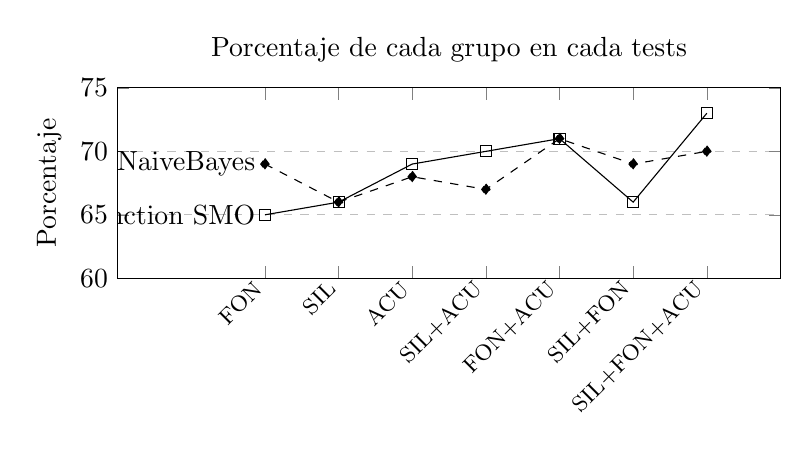
\begin{tikzpicture}

\begin{axis}[
    title={Porcentaje de cada grupo en cada tests},
    ylabel={Porcentaje},
    xmin=-1, xmax=8,
    ymin=60, ymax=75,
    xtick={1,2,3,4,5,6,7},
    xticklabels={FON,SIL,ACU,SIL+ACU,FON+ACU,SIL+FON, SIL+FON+ACU},
    x tick label style={rotate=45, anchor=east, font=\footnotesize},
    ytick={60,65,70,75},
    ymajorgrids=true,
    grid style=dashed,
] 

\addplot[mark=diamond*,dashed]coordinates {
    (1,69)(2,66)(3,68)(4,67)(5,71)(6,69)(7,70) };
\addplot[mark=square,solid,]coordinates {
    (1,65)(2,66)(3,69)(4,70)(5,71)(6,66)(7,73) };

\node [left] at (axis cs: 1, 69) {NaiveBayes};
\node [left] at (axis cs: 1, 65) {Function SMO};

\end{axis}
\end{tikzpicture}

Lo esperable es que aumentando los atributos se aumente el porcentaje de clasificación. Esta idea se comprueba ya que la combinación que obtuvo mejor porcentaje fue $SIL+FON+ACU$ para el clasificador Function SMO. En segundo lugar salió la combinación de $FON+ACU$ para ambos clasificadores y en tercero $SIL+ACU$ sólo para Function SMO. 

Podemos notar que el tipo de atributo que posee mayor presencia son los atributos acústicos, ya que se encuentran en los tres primeros grupos que obtuvieron mejor porcentaje. Quizás individualmente no tengan un atributo con mucha información predominante, pero la combinación de todos los atributos de esa clase hace que los clasificadores tengan buenas métricas.